\label{fnt2.2.1-8}

\begin{wrapfigure}{R}{.28\textwidth}
	\vspace{-15pt}
  	\centering
	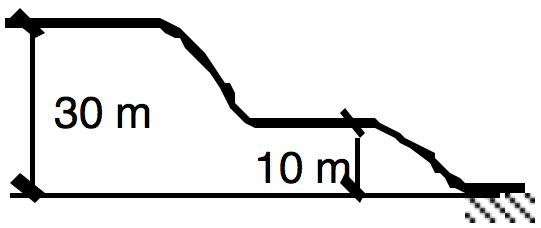
\includegraphics[width=0.95\linewidth]{fnt221-8-hill}
	\vspace{-10pt}
\end{wrapfigure}

A skier (of mass \unit[55]{kg}) skies down the smooth (frictionless) ski slope illustrated in the cross-sectional diagram. She pushes off at the top with a speed of \unitfrac[10]{m}{s}. At the bottom (\unit[0]{m}), she comes to a stop by digging her skis in sideways.

\begin{enumerate}[(a)]
	\item\label{fnt2.2.1-8a} Construct a complete \EnergyDiagram{} that can be used to predict the speed of the skier when she is on the middle flat part (at \unit[10]{m}). Substitute all known values of constants and variables, and identify any unknown(s). Do you have enough information to determine the speed at this part of the hill?

	
	\item\label{fnt2.2.1-8b} Construct a complete \EnergyDiagram{} that can be used to predict the skier's maximum speed just before digging in her skis at the bottom. Substitute for constants and variables and identify any unknown(s) as in Part~\eqref{fnt2.2.1-8a}.

	
	\item\label{fnt2.2.1-8c} Assuming that the snow at the point where she comes to a stop is at a temperature of \unit[0]{\textdegree{}C} and that all of the kinetic energy of the skier goes into melting the snow, construct a complete \EnergyDiagram{} that can be used to predict the amount of snow melted by the skier while stopping. Substitute for constants and variables and identify any unknown(s) as in Part~\eqref{fnt2.2.1-8a}.
\end{enumerate}
